\chapter{التركيز والتخفيف}\label{ch:g10:concentration-and-dilution}

كيس \omterm{def:g2:mixing-and-dissolving:dissolve}{محلول} وريدي معلّق فوق سرير مريض. يقول ملصقه «كلوريد الصوديوم
0.9 \%»: ملح في ماء، لا أكثر. لكن العدد 0.9 ليس تفصيلًا. فلو قلّ الملح
لانتفخت خلايا دم المريض بالماء؛ ولو زاد لانكمشت. \omterm{def:g2:mixing-and-dissolving:dissolve}{فالمحلول} لا يوصف بمكوناته
وحدها، بل بمقدار \omterm{def:g6:solutions-and-solubility:solute}{المذاب} الذي يحويه كل حجم منه، أي بتركيزه. يقيس هذا الفصل
التراكيز، ويحضّر محاليل ذات تركيز دقيق، ويخففها.

\begin{recall}
يتكوّن \omterm{def:g2:mixing-and-dissolving:dissolve}{المحلول} من \omterm{def:g6:solutions-and-solubility:solute}{مذيب} \omterm{def:g6:solutions-and-solubility:solute}{ومذاب} ذائب أو أكثر؛ \omterm{def:g6:solutions-and-solubility:solubility}{والذوبانية} أكبر كتلة من \omterm{def:g6:solutions-and-solubility:solute}{المذاب}
يستطيع مقدار معيّن من \omterm{def:g6:solutions-and-solubility:solute}{المذيب} أن يذيبها (\cref{ch:g6:solutions-and-solubility}).
\omterm{def:g10:the-mole:amount}{وكمية مادة} \omterm{def:g6:pure-substances-and-mixtures:species}{نوع كيميائي} هي $n = m/M$، \omterm{def:g10:the-mole:amount}{بالمول} (\cref{ch:g10:the-mole}).
\end{recall}

\begin{omfigure}
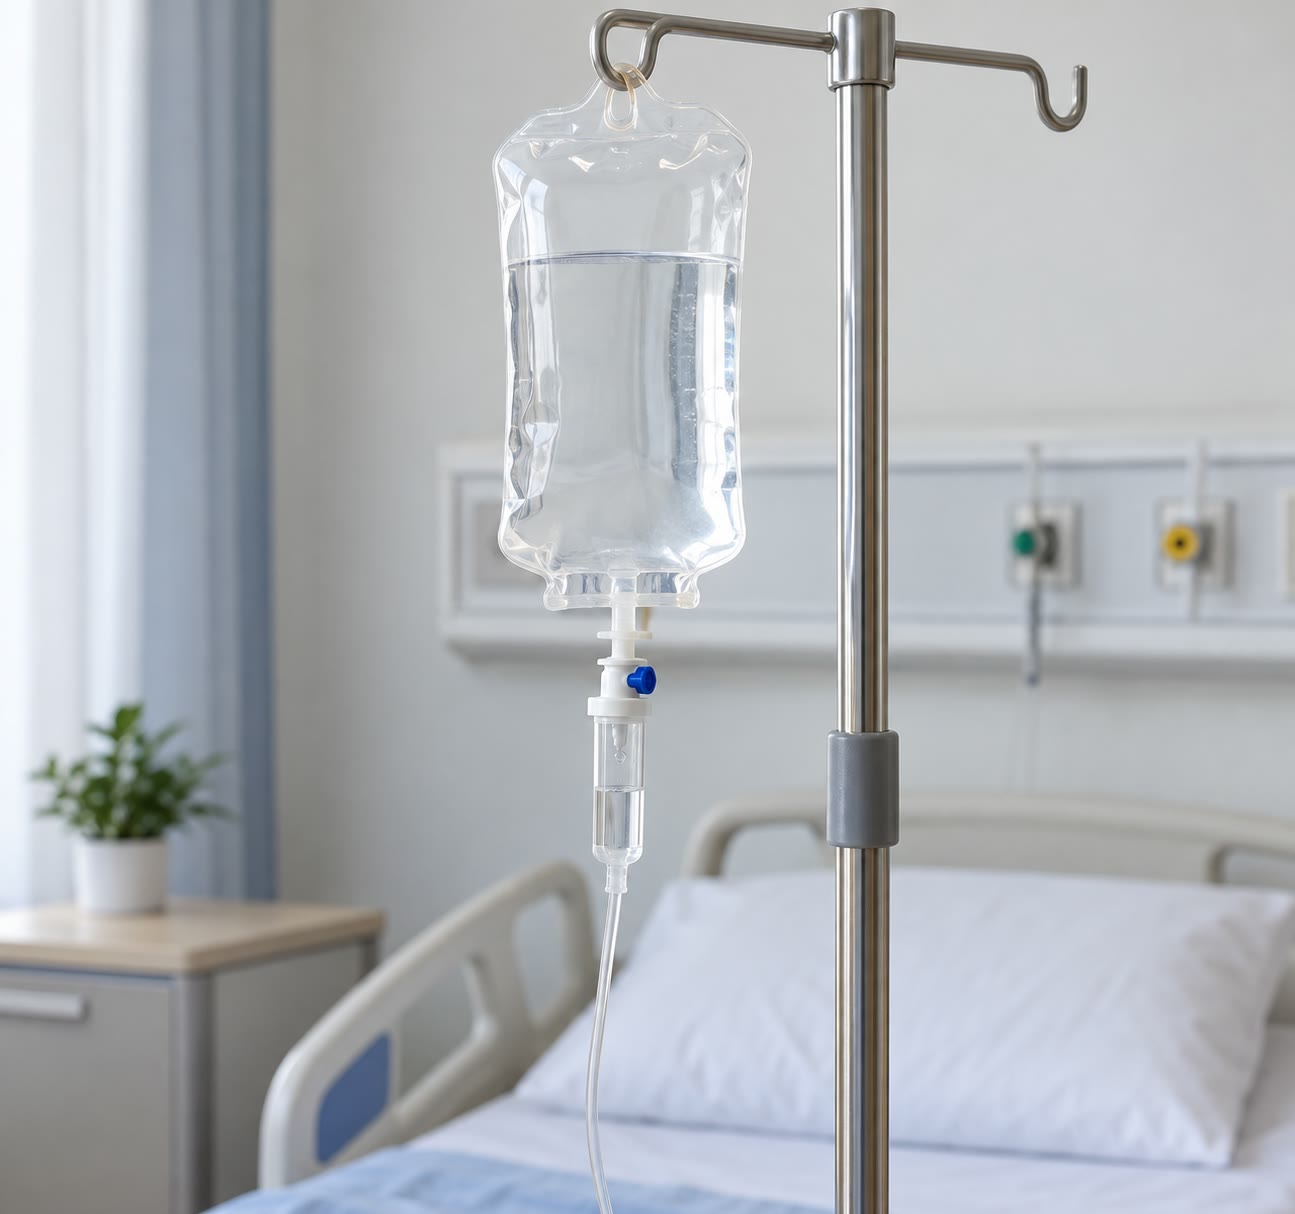
\includegraphics[width=0.42\linewidth]{images/book1/ai/g10-drip-bag.jpg}

{\small كيس \omterm{def:g2:mixing-and-dissolving:dissolve}{محلول} ملحي وريدي: يجب أن يكون التركيز صحيحًا.}
\end{omfigure}

\section{التركيز الكتلي}

\begin{definition}[التركيز الكتلي]\label{def:g10:concentration-and-dilution:mass-concentration}
\emph{التركيز الكتلي}\index{تركيز كتلي} $C_m$ \omterm{def:g6:solutions-and-solubility:solute}{لمذاب} في \omterm{def:g2:mixing-and-dissolving:dissolve}{محلول} هو كتلة \omterm{def:g6:solutions-and-solubility:solute}{المذاب}
الذائب لكل حجم من \omterm{def:g2:mixing-and-dissolving:dissolve}{المحلول}:
\[
  C_m = \frac{m_{\text{المذاب}}}{V_{\text{المحلول}}},
\]
بالغرام لكل لتر (\si{g/L}).
\end{definition}

\begin{example}[الماء المحلّى]\label{ex:g10:concentration-and-dilution:sugar}
تُذاب \qty{20}{g} من السكر في الماء، ويُكمَّل \omterm{def:g2:mixing-and-dissolving:dissolve}{المحلول} حتى
\qty{0.50}{L}. فتركيزه الكتلي من السكر
$C_m = \qty{20}{g} / \qty{0.50}{L} = \qty{40}{g/L}$. ولأي جزء منه التركيز
نفسه: فكأس منه حجمها \qty{0.20}{L} تحوي
$\qty{40}{g/L} \times \qty{0.20}{L} = \qty{8.0}{g}$ من السكر.
\end{example}


\begin{remark}[الحجم هو حجم المحلول]\label{rem:g10:concentration-and-dilution:volume}
الحجم في $C_m$ هو حجم \omterm{def:g2:mixing-and-dissolving:dissolve}{المحلول} كله، لا حجم الماء المصبوب: فإذابة \omterm{def:g6:solutions-and-solubility:solute}{المذاب} تغيّر
الحجم قليلًا. ولهذا \emph{يُكمَّل} \omterm{def:g2:mixing-and-dissolving:dissolve}{المحلول} دائمًا حتى حجم نهائي معلوم، في
حوجلة معلَّمة لذلك.
\end{remark}

\begin{remark}[التركيز ليس الذوبانية]\label{rem:g10:concentration-and-dilution:not-solubility}
% ledger: sol:NaCl, saline:NaCl
\omterm{def:g6:solutions-and-solubility:solubility}{ذوبانية} \omterm{def:g6:solutions-and-solubility:solute}{المذاب} هي \emph{أكبر} تركيز يمكن أن يبلغه؛ وقد يكون \omterm{def:g2:mixing-and-dissolving:dissolve}{للمحلول} أي تركيز
من الصفر حتى هذه القيمة. فكلوريد الصوديوم \omterm{def:g2:mixing-and-dissolving:dissolve}{يذوب} حتى نحو \qty{360}{g} في
الكيلوغرام من الماء عند \qty{25}{\celsius}؛ بينما لا يحوي الكيس الوريدي إلا
\qty{9}{g} في اللتر، أي بعيدًا جدًا عن الإشباع.
\end{remark}

\begin{remark}[النسب المئوية على الملصقات]\label{rem:g10:concentration-and-dilution:percent}
% ledger: saline:NaCl
على الملصقات الطبية والغذائية، تعني «0.9 \%» لجسم صلب \omterm{def:g6:solutions-and-solubility:solute}{مذاب} في الماء عادة
\qty{0.9}{g} من \omterm{def:g6:solutions-and-solubility:solute}{المذاب} في \qty{100}{mL} من \omterm{def:g2:mixing-and-dissolving:dissolve}{المحلول}. وبالغرام لكل لتر تكون
أكبر بعشر مرات: فالكيس الوريدي يحوي \qty{9.0}{g/L} من كلوريد
الصوديوم.
\end{remark}

\section{التركيز المولي}

\begin{definition}[التركيز المولي]\label{def:g10:concentration-and-dilution:molar-concentration}
\emph{التركيز المولي}\index{تركيز مولي} $c$ \omterm{def:g6:solutions-and-solubility:solute}{لمذاب} في \omterm{def:g2:mixing-and-dissolving:dissolve}{محلول} هو \omterm{def:g10:the-mole:amount}{كمية مادة}
\omterm{def:g6:solutions-and-solubility:solute}{المذاب} الذائب لكل حجم من
\omterm{def:g2:mixing-and-dissolving:dissolve}{المحلول}:
\[
  c = \frac{n_{\text{المذاب}}}{V_{\text{المحلول}}},
\]
\omterm{def:g10:the-mole:amount}{بالمول} لكل لتر (\si{mol/L}).
\end{definition}

\begin{proposition}[من تركيز إلى آخر]\label{prop:g10:concentration-and-dilution:link}
\omterm{def:g6:solutions-and-solubility:solute}{لمذاب} كتلته المولية $M$،
\[
  C_m = c \times M .
\]
\end{proposition}

\begin{proof}
$C_m = m / V = (n \times M) / V = (n / V) \times M = c \times M$.
\end{proof}

\begin{example}[الكيس الوريدي بالمولات]\label{ex:g10:concentration-and-dilution:drip}
% ledger: saline:NaCl, saline:Na, aw:Na, aw:Cl
يحوي الكيس الوريدي \qty{9.0}{g/L} من كلوريد الصوديوم، وكتلته المولية
\qty{58.5}{g/mol}. فتركيزه المولي
\[
  c = \frac{C_m}{M} = \frac{\qty{9.0}{g/L}}{\qty{58.5}{g/mol}}
    = \qty{0.154}{mol/L}.
\]
ويعطي ملصق الصانع العدد نفسه بالطريقة المعاكسة: 154 جزءًا من ألف من \omterm{def:g10:the-mole:amount}{المول}
من \omterm{def:g9:ions:ion}{أيونات} الصوديوم في كل لتر.
\end{example}

\begin{remark}[الأيونات في المحلول]\label{rem:g10:concentration-and-dilution:ions}
\omterm{def:g2:mixing-and-dissolving:dissolve}{يذوب} كلوريد الصوديوم \omterm{def:g9:ions:ion}{أيونات} منفصلة \ce{Na+} و\ce{Cl-}
(\cref{ch:g9:ions}): \omterm{def:g2:mixing-and-dissolving:dissolve}{فمحلول} كلوريد الصوديوم الذي تركيزه \qty{0.154}{mol/L}
يحوي \qty{0.154}{mol/L} من \omterm{def:g9:ions:ion}{أيونات} الصوديوم و\qty{0.154}{mol/L} من \omterm{def:g9:ions:ion}{أيونات}
الكلوريد. أما كيف يتفكك الجسم الصلب الأيوني في الماء فموضوع
فصل لاحق.
\end{remark}

\begin{omfigure}
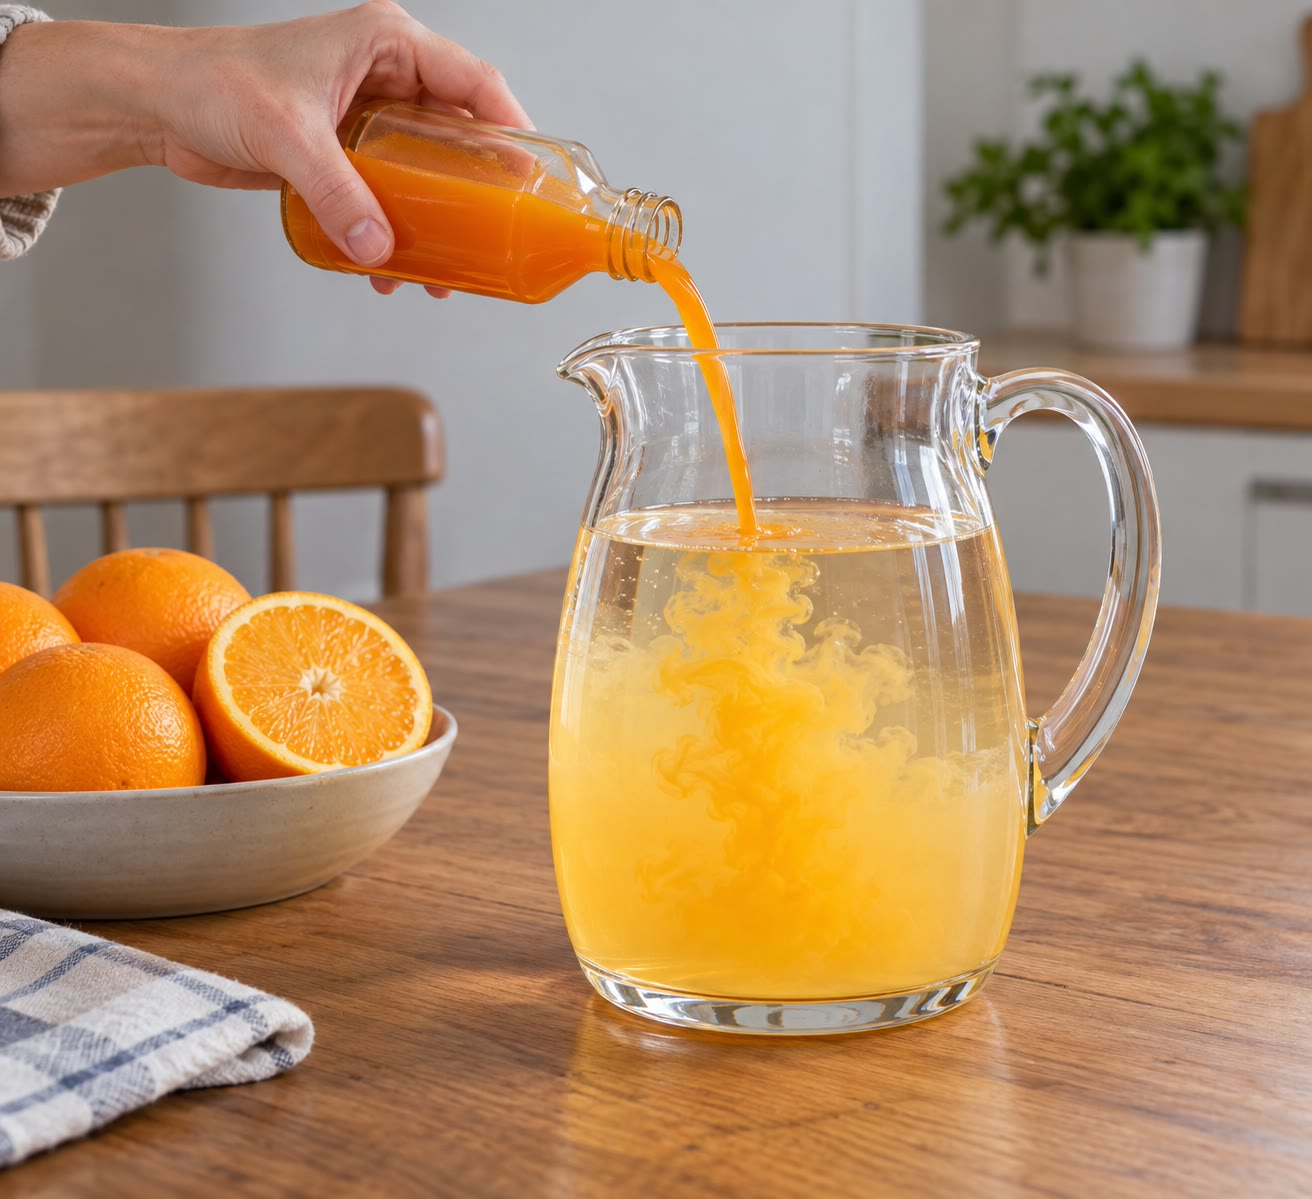
\includegraphics[width=0.45\linewidth]{images/book1/ai/g10-squash-jug.jpg}

{\small شراب الفاكهة المركّز يُخفَّف بالماء في إبريق: فيحوي المشروب المقدار نفسه من
شراب الفاكهة، في حجم أكبر.}
\end{omfigure}

\section{تحضير محلول بالإذابة}

\begin{method}[تحضير محلول بإذابة جسم صلب]\label{met:g10:concentration-and-dilution:dissolving}
لتحضير حجم $V$ من \omterm{def:g2:mixing-and-dissolving:dissolve}{محلول} تركيزه المولي $c$:
\begin{enumerate}
  \item احسب \omterm{def:g10:the-mole:amount}{كمية المادة} اللازمة، $n = c \times V$، والكتلة الواجب
        وزنها، $m = n \times M$.
  \item زن هذه الكتلة من الجسم الصلب في صحن صغير على ميزان.
  \item صب الجسم الصلب عبر قمع في حوجلة معيارية حجمها
        $V$؛ واشطف الصحن والقمع بالماء المقطر في الحوجلة، حتى لا
        يضيع شيء من الجسم الصلب.
  \item أضف الماء المقطر حتى نصف الحوجلة تقريبًا وحرّكها دائريًا حتى
        \omterm{def:g2:mixing-and-dissolving:dissolve}{يذوب} الجسم الصلب كله.
  \item أضف الماء المقطر حتى الخط المعلَّم، والقطرات الأخيرة بالقطارة؛
        ثم سدّ الحوجلة واقلبها عدة مرات \omterm{def:g2:mixing-and-dissolving:mix}{للخلط}.
\end{enumerate}
\end{method}

\begin{omfigure}
\begin{tikzpicture}[font=\small, scale=1.05]
  % 1. weigh
  \pic[transform shape] at (0,0) {balance};
  \fill[black!8, draw=black!55] (-0.45,0.8) -- (0.45,0.8) -- (0.38,0.98)
    -- (-0.38,0.98) -- cycle;
  \fill[white, draw=black!40] (-0.25,0.98) .. controls (-0.1,1.15) and
    (0.1,1.15) .. (0.25,0.98) -- cycle;
  \node[align=center, anchor=north] at (0,-0.2) {\foreignlanguage{arabic}{\babelsublr{1.} زن}\\ الجسم الصلب};
  % 2. transfer through a funnel
  \pic[transform shape] at (3.2,0) {volflask={0.08}{omWater}};
  \pic[transform shape] at (3.2,3.0) {funnel};
  \draw[omProp, thick, -{Stealth}] (2.4,5.0) -- (2.85,4.65);
  \node[align=center, anchor=north] at (3.2,-0.2) {\foreignlanguage{arabic}{\babelsublr{2.} انقل،}\\ واشطف فيها};
  % 3. half full, swirl
  \pic[transform shape] at (6.4,0) {volflask={0.45}{omWater}};
  \draw[omProp, thick, -{Stealth}] (5.55,0.5) arc[start angle=200,
    end angle=340, x radius=0.9, y radius=0.3];
  \node[align=center, anchor=north] at (6.4,-0.2) {\foreignlanguage{arabic}{\babelsublr{3.} حتى النصف:}\\ حرّك لتذيب};
  % 4. to the mark
  \pic[transform shape] at (9.6,0) {volflask={1}{omWater}};
  \fill[black!45] (9.43,3.6) rectangle (9.77,3.85);
  \draw[omDef, thick, <-] (9.82,2.9) -- (10.6,3.3) node[right] {الخط المعلَّم};
  \node[align=center, anchor=north] at (9.6,-0.2) {\foreignlanguage{arabic}{\babelsublr{4.} املأ حتى الخط،}\\
    وسدّ، واخلط};
\end{tikzpicture}

{\small تحضير \omterm{def:g2:mixing-and-dissolving:dissolve}{محلول} بإذابة جسم صلب: الوزن، والنقل، والإذابة، ثم الإكمال حتى خط
الحوجلة المعيارية.}
\end{omfigure}

\begin{inthelab}[الملء حتى الخط المعلَّم]
خط الحوجلة المعيارية حلقة حول عنقها. والماء في أنبوب زجاجي ضيق لا ينتهي
بسطح مستوٍ: بل ينحني سطحه نحو الأسفل في الوسط، مكوّنًا هلالًا. وتكون الحوجلة
ممتلئة حين يلامس \emph{أسفل} الهلال الخط، والعين على مستوى الخط، بحيث يبدو
مقدَّم الحلقة ومؤخَّرها خطًا واحدًا. فإذا نُظر من أعلى أو من أسفل قد يبدو
المستوى صحيحًا وهو ليس كذلك.
\end{inthelab}

\begin{omfigure}
\begin{tikzpicture}[font=\small]
  \newcommand{\neck}[2]{% x, meniscus bottom height
    \fill[omWater] (#1-0.5,0) -- (#1-0.5,{#2+0.25}) .. controls
      (#1-0.25,#2) and (#1+0.25,#2) .. (#1+0.5,{#2+0.25}) -- (#1+0.5,0) -- cycle;
    \draw[black!60, line width=0.8pt] (#1-0.5,0) -- (#1-0.5,3);
    \draw[black!60, line width=0.8pt] (#1+0.5,0) -- (#1+0.5,3);
    \draw[omDef, line width=0.9pt] (#1-0.5,1.5) -- (#1+0.5,1.5);
    \draw[black!50] (#1-0.5,{#2+0.25}) .. controls (#1-0.25,#2) and
      (#1+0.25,#2) .. (#1+0.5,{#2+0.25});}
  \newcommand{\eye}[2]{% x, y: an eye looking to the right
    \draw[black!70] (#1-0.25,#2) .. controls (#1-0.1,#2+0.18) and
      (#1+0.1,#2+0.18) .. (#1+0.2,#2) .. controls (#1+0.1,#2-0.18) and
      (#1-0.1,#2-0.18) .. (#1-0.25,#2);
    \fill[black!70] (#1+0.05,#2) circle (0.06);}
  % right
  \neck{1.5}{1.5}
  \eye{-0.4}{1.5}
  \draw[dashed, black!50] (-0.1,1.5) -- (2.4,1.5);
  \node[align=center] at (1.5,-0.55) {صحيح: العين في المستوى،\\ وأسفل الهلال على الخط};
  % too high
  \neck{6}{1.85}
  \eye{4.1}{1.85}
  \draw[dashed, black!50] (4.4,1.85) -- (6.9,1.85);
  \node[align=center] at (6,-0.55) {ماء زائد:\\ الهلال فوق الخط};
  % too low
  \neck{10.5}{0.85}
  \eye{8.6}{0.85}
  \draw[dashed, black!50] (8.9,0.85) -- (11.4,0.85);
  \node[align=center] at (10.5,-0.55) {ماء ناقص:\\ الهلال تحت الخط};
\end{tikzpicture}

{\small عنق حوجلة معيارية، مكبَّرًا ومنظورًا إليه والعين على مستوى الهلال.
والخط الأزرق هو الخط المعلَّم. والحوجلة اليسرى وحدها مملوءة على النحو
الصحيح.}
\end{omfigure}

\section{التخفيف}

\begin{definition}[التخفيف، والمحلول الأم، ومعامل التخفيف]\label{def:g10:concentration-and-dilution:dilution}
\emph{التخفيف}\index{تخفيف} يخفض تركيز \omterm{def:g2:mixing-and-dissolving:dissolve}{محلول} بإضافة \omterm{def:g6:solutions-and-solubility:solute}{المذيب}. \omterm{def:g2:mixing-and-dissolving:dissolve}{والمحلول} المركّز
المأخوذ في البداية هو \emph{المحلول الأم}\index{محلول أم}. و\emph{معامل
التخفيف}\index{معامل التخفيف} $F$ هو نسبة تركيز \omterm{def:g2:mixing-and-dissolving:dissolve}{المحلول} الأم إلى تركيز
\omterm{def:g2:mixing-and-dissolving:dissolve}{المحلول} المخفف:
\[
  F = \frac{c_{\text{الأم}}}{c_{\text{المخفف}}} .
\]
\end{definition}

\begin{proposition}[كمية المذاب محفوظة]\label{prop:g10:concentration-and-dilution:kept}
في أثناء \omterm{def:g10:concentration-and-dilution:dilution}{التخفيف} لا تتغير \omterm{def:g10:the-mole:amount}{كمية مادة} \omterm{def:g6:solutions-and-solubility:solute}{المذاب}: فإذا أُكمل حجم $V_0$ من \omterm{def:g10:concentration-and-dilution:dilution}{محلول أم}
تركيزه $c_0$ حتى حجم $V_1$، كان \omterm{def:g2:mixing-and-dissolving:dissolve}{للمحلول} المخفف التركيز $c_1$ المعطى
بالعلاقة
\[
  c_0 \times V_0 = c_1 \times V_1,
  \qquad\text{إذن}\qquad
  F = \frac{c_0}{c_1} = \frac{V_1}{V_0} .
\]
وكذلك الأمر في التراكيز الكتلية.
\end{proposition}

\begin{proof}
لا يُضاف إلا \omterm{def:g6:solutions-and-solubility:solute}{المذيب}: \omterm{def:g6:solutions-and-solubility:solute}{فالمذاب} المأخوذ مع الحجم $V_0$، وكميته
$c_0 V_0$، موجود كله في الحجم النهائي $V_1$، حيث يكوّن \omterm{def:g10:the-mole:amount}{كمية
المادة} $c_1 V_1$.
\end{proof}


\begin{method}[تحضير محلول بالتخفيف]\label{met:g10:concentration-and-dilution:diluting}
لتحضير حجم $V_1$ من \omterm{def:g2:mixing-and-dissolving:dissolve}{محلول} تركيزه $c_1$ انطلاقًا من \omterm{def:g10:concentration-and-dilution:dilution}{محلول أم}
تركيزه $c_0$:
\begin{enumerate}
  \item احسب حجم \omterm{def:g10:concentration-and-dilution:dilution}{المحلول الأم} الواجب أخذه،
        $V_0 = c_1 V_1 / c_0$ (أي $V_1 / F$).
  \item صب قليلًا من \omterm{def:g10:concentration-and-dilution:dilution}{المحلول الأم} في كأس نظيفة (ولا تسحب بالماصّة مباشرة
        من القارورة أبدًا) وخذ بالضبط $V_0$ بماصّة
        معيارية، مملوءة حتى خطها.
  \item أفرغ الماصّة في حوجلة معيارية حجمها $V_1$.
  \item أضف الماء المقطر حتى الخط المعلَّم، ثم سدّ واخلط.
\end{enumerate}
\end{method}

\begin{example}[تخفيف بعشرة أضعاف]\label{ex:g10:concentration-and-dilution:tenfold}
\omterm{def:g10:concentration-and-dilution:dilution}{محلول أم} من كبريتات النحاس تركيزه $c_0 = \qty{0.10}{mol/L}$؛ ويلزم
\qty{100.0}{mL} بتركيز $c_1 = \qty{0.010}{mol/L}$. \omterm{def:g10:concentration-and-dilution:dilution}{فمعامل التخفيف}
$F = 0.10 / 0.010 = 10$، إذن $V_0 = \qty{100.0}{mL} / 10 =
\qty{10.0}{mL}$: ماصّة من \qty{10.0}{mL} وحوجلة من \qty{100.0}{mL}.
\end{example}

\begin{omfigure}
\begin{tikzpicture}[font=\small, scale=0.85]
  % 1. take the stock with a pipette
  \pic[transform shape] at (0,0) {beaker={0.6}{cyan!70!blue!55}};
  \pic[transform shape] at (0,0.2) {pipette={1}{cyan!70!blue!55}};
  \node[align=center, anchor=north] at (0,-0.2) {\foreignlanguage{arabic}{\babelsublr{1.} اسحب $V_0$}\\ من المحلول الأم};
  \draw[omProp, very thick, -{Stealth}] (1.3,2.6) -- (2.6,2.6);
  % 2. empty it into the flask
  \pic[transform shape] at (4,0) {volflask={0.22}{cyan!70!blue!55}};
  \pic[transform shape] at (4,2.6) {pipette={0.12}{cyan!70!blue!55}};
  \node[align=center, anchor=north] at (4,-0.2) {\foreignlanguage{arabic}{\babelsublr{2.} أفرغها في}\\ الحوجلة};
  \draw[omProp, very thick, -{Stealth}] (5.3,2.6) -- (6.6,2.6);
  % 3. water to the mark
  \pic[transform shape] at (8,0) {volflask={1}{cyan!70!blue!14}};
  \draw[omDef, thick, <-] (8.2,2.9) -- (9.1,3.4) node[right] {الخط المعلَّم};
  \node[align=center, anchor=north] at (8,-0.2) {\foreignlanguage{arabic}{\babelsublr{3.} الماء حتى الخط:}\\
    \foreignlanguage{arabic}{الحجم $V_1$}};
\end{tikzpicture}

{\small \omterm{def:g10:concentration-and-dilution:dilution}{التخفيف}: حجم $V_0$ من \omterm{def:g10:concentration-and-dilution:dilution}{المحلول الأم}، يُقاس بماصّة، يُكمَّل حتى $V_1$
في حوجلة معيارية. ويبهت اللون بقدر \omterm{def:g10:concentration-and-dilution:dilution}{معامل التخفيف}
$V_1 / V_0$.}
\end{omfigure}

\section{السلّم المرجعي}

\begin{definition}[المحلول المعياري والسلّم المرجعي]\label{def:g10:concentration-and-dilution:standard}
\emph{المحلول المعياري}\index{محلول معياري} \omterm{def:g2:mixing-and-dissolving:dissolve}{محلول} تركيزه معروف بدقة.
و\emph{السلّم المرجعي}\index{سلم مرجعي} سلسلة من المحاليل المعيارية \omterm{def:g6:solutions-and-solubility:solute}{للمذاب}
نفسه، بتراكيز متزايدة، تُحضَّر عادة \omterm{def:g10:concentration-and-dilution:dilution}{بتخفيف} \omterm{def:g10:concentration-and-dilution:dilution}{محلول أم} واحد؛ ومقارنة \omterm{def:g2:mixing-and-dissolving:dissolve}{محلول} مجهول
به تعطي تقديرًا لتركيز المجهول.
\end{definition}

\begin{example}[سلّم أزرق]\label{ex:g10:concentration-and-dilution:scale}
انطلاقًا من \omterm{def:g10:concentration-and-dilution:dilution}{محلول أم} من كبريتات النحاس تركيزه \qty{0.20}{mol/L} تُحضَّر ستة
محاليل معيارية بالتراكيز 0.02 و0.04 و0.06 و0.08 و0.10
و\qty{0.12}{mol/L}، كل منها في أنبوب مماثل مملوء حتى الارتفاع نفسه.
\omterm{def:g2:mixing-and-dissolving:dissolve}{ومحلول} مجهول التركيز، في أنبوب من النوع نفسه، يبدو أدكن من أنبوب
\qty{0.06}{mol/L} وأبهت من أنبوب
\qty{0.08}{mol/L}: فتركيزه يقع بينهما، أي نحو
\qty{0.07}{mol/L}.
\end{example}

\begin{omfigure}
\begin{tikzpicture}[font=\small]
  \foreach \i/\c/\p in {0/0.02/8, 1/0.04/16, 2/0.06/24, 3/0.08/32,
                        4/0.10/40, 5/0.12/48} {
    \pic at (1.2*\i,0) {testtube={0.75}{cyan!70!blue!\p}};
    \node[anchor=north] at (1.2*\i,-0.15) {\c};
  }
  \pic at (8.4,0) {testtube={0.75}{cyan!70!blue!28}};
  \node[anchor=north] at (8.4,-0.15) {?};
  \draw[black!40] (7.55,-0.6) -- (7.55,3.2);
  \node[anchor=north] at (3,-0.7) {\foreignlanguage{arabic}{التركيز \babelsublr{(\si{mol/L})}}};
  \node[anchor=north] at (8.4,-0.7) {المجهول};
\end{tikzpicture}

{\small سلّم مرجعي من محاليل كبريتات النحاس \omterm{def:g2:mixing-and-dissolving:dissolve}{ومحلول} مجهول. يقع المجهول بين
الأنبوبين الثالث والرابع.}
\end{omfigure}

\begin{safety}{\ghs[0.82cm]{GHS05}\ghs[0.82cm]{GHS07}\ghs[0.82cm]{GHS09}}
% ledger: ghs:CuSO4
محاليل كبريتات النحاس: ضارة إذا ابتُلعت، ومهيّجة للجلد، ومؤذية للعينين،
وشديدة السمية للأحياء المائية. نظارات واقية وقفازات؛ وتُجمع المحاليل المستعملة
لمعالجتها، ولا تُصب أبدًا في المغسلة.
\end{safety}

\begin{remark}[حدود العين]\label{rem:g10:concentration-and-dilution:eye}
لا تستطيع العين أن تقول إلا «بين هذين الأنبوبين». ولقياس تركيز \omterm{def:g2:mixing-and-dissolving:dissolve}{محلول} بدقة
أكبر من لونه، يقيس الكيميائيون مقدار الضوء الذي يمتصه؛ وهذا بالضبط ما يفعله
فصل لاحق.
\end{remark}

\section{تمارين}

\begin{exercise}[$\star$]\label{exo:g10:concentration-and-dilution:1}
تُذاب \qty{5.0}{g} من السكر لتحضير \qty{250}{mL} من \omterm{def:g2:mixing-and-dissolving:dissolve}{المحلول}.
احسب \omterm{def:g10:concentration-and-dilution:mass-concentration}{التركيز الكتلي} للسكر بالغرام لكل لتر.
\end{exercise}

\begin{exercise}[$\star$]\label{exo:g10:concentration-and-dilution:2}
\omterm{def:g2:mixing-and-dissolving:dissolve}{محلول} حجمه \qty{200}{mL} يحوي \qty{0.050}{mol} من الغلوكوز.
احسب تركيزه المولي.
\end{exercise}

\begin{exercise}[$\star$]\label{exo:g10:concentration-and-dilution:3}
ما كتلة كبريتات النحاس اللامائية \ce{CuSO4} الواجب وزنها لتحضير
\qty{100.0}{mL} من \omterm{def:g2:mixing-and-dissolving:dissolve}{محلول} تركيزه \qty{0.10}{mol/L}؟
\end{exercise}

\begin{exercise}[$\star$]\label{exo:g10:concentration-and-dilution:4}
\omterm{def:g10:concentration-and-dilution:dilution}{محلول أم} تركيزه \qty{1.0}{mol/L} يُخفَّف إلى \qty{0.050}{mol/L}.
ما \omterm{def:g10:concentration-and-dilution:dilution}{معامل التخفيف}؟ وما حجم \omterm{def:g10:concentration-and-dilution:dilution}{المحلول الأم} اللازم لتحضير
\qty{100.0}{mL} من \omterm{def:g2:mixing-and-dissolving:dissolve}{المحلول} المخفف؟
\end{exercise}

\begin{exercise}[$\star$]\label{exo:g10:concentration-and-dilution:5}
\omterm{def:g2:mixing-and-dissolving:dissolve}{محلول} من كلوريد الصوديوم تركيزه المولي
\qty{0.10}{mol/L}. ما تركيزه الكتلي؟
\end{exercise}

\begin{exercise}[$\star\star$]\label{exo:g10:concentration-and-dilution:6}
ما حجم \omterm{def:g10:concentration-and-dilution:dilution}{محلول أم} تركيزه \qty{0.50}{mol/L} الواجب أخذه لتحضير
\qty{250.0}{mL} من \omterm{def:g2:mixing-and-dissolving:dissolve}{محلول} تركيزه \qty{0.020}{mol/L}؟ سمِّ قطعتي الأدوات
الزجاجية المستعملتين.
\end{exercise}

\begin{exercise}[$\star\star$]\label{exo:g10:concentration-and-dilution:7}
لماذا يُحضَّر \omterm{def:g2:mixing-and-dissolving:dissolve}{محلول} ذو تركيز دقيق في حوجلة معيارية لا في كأس مدرّجة؟ ولماذا
يُقاس حجم من \omterm{def:g10:concentration-and-dilution:dilution}{المحلول الأم} بماصّة معيارية لا بمخبار
مدرّج؟
\end{exercise}

\begin{exercise}[$\star\star$]\label{exo:g10:concentration-and-dilution:8}
انظر إلى \omterm{def:g10:concentration-and-dilution:standard}{السلّم المرجعي} لكبريتات النحاس. \omterm{def:g2:mixing-and-dissolving:dissolve}{محلول} مجهول ثانٍ أبهت من أنبوب
\qty{0.04}{mol/L} لكنه أدكن من أنبوب
\qty{0.02}{mol/L}. قدّر تركيزه. وكيف يمكن تغيير السلّم لتقديره بدقة
أكبر؟
\end{exercise}

\begin{exercise}[$\star\star$]\label{exo:g10:concentration-and-dilution:9}
\omterm{def:g2:mixing-and-dissolving:dissolve}{محلول} غلوكوز للحقن يحوي \qty{50}{g/L} من الغلوكوز
\ce{C6H12O6}. احسب تركيزه المولي.
\end{exercise}

\begin{exercise}[$\star\star$]\label{exo:g10:concentration-and-dilution:10}
يُحضَّر شراب بإذابة \qty{342}{g} من السكروز \ce{C12H22O11} لتحضير
\qty{1.00}{L} من \omterm{def:g2:mixing-and-dissolving:dissolve}{المحلول}. احسب تركيزه المولي. ثم يُخفَّف عشر مرات. ما كتلة
السكروز في ملعقة من \qty{20}{mL} من الشراب
المخفف؟
\end{exercise}

\begin{exercise}[$\star\star$]\label{exo:g10:concentration-and-dilution:11}
\omterm{def:g2:mixing-and-dissolving:dissolve}{محلول} تركيزه الكتلي \qty{12}{g/L}. ما تركيزه (أ) بعد إضافة ماء يضاعف حجمه؛
(ب) بعد \omterm{def:g3:separating-mixtures:evaporate}{تبخير} نصف مائه، مع بقاء \omterm{def:g6:solutions-and-solubility:solute}{المذاب} كله
ذائبًا؟
\end{exercise}

\begin{exercise}[$\star\star\star$]\label{exo:g10:concentration-and-dilution:12}
\omterm{def:g2:mixing-and-dissolving:dissolve}{محلول} تركيزه \qty{0.10}{mol/L} يُخفَّف عشر مرات، ثم تُخفَّف النتيجة عشر مرات
أخرى، ثم مرة أخرى.
\begin{enumerate}
  \item ما التركيز النهائي؟
  \item لماذا يُفعل ذلك في ثلاث خطوات لا في \omterm{def:g10:concentration-and-dilution:dilution}{تخفيف} واحد بألف
        ضعف (فكّر في أحجام الأدوات الزجاجية اللازمة)؟
\end{enumerate}
\end{exercise}

\begin{exercise}[$\star\star\star$]\label{exo:g10:concentration-and-dilution:13}
تُذاب \qty{11.1}{g} من كلوريد الكالسيوم \ce{CaCl2} لتحضير
\qty{500.0}{mL} من \omterm{def:g2:mixing-and-dissolving:dissolve}{المحلول}. وفي الماء يتفكك الجسم الصلب إلى \omterm{def:g9:ions:ion}{أيونات} كالسيوم
\ce{Ca^2+} \omterm{def:g9:ions:ion}{وأيونات} كلوريد \ce{Cl-}.
\begin{enumerate}
  \item احسب \omterm{def:g10:concentration-and-dilution:molar-concentration}{التركيز المولي} لكلوريد الكالسيوم \omterm{def:g6:solutions-and-solubility:solute}{المذاب}.
  \item استنتج التركيزين الموليين \omterm{def:g9:ions:ion}{لأيونات} الكالسيوم ولأيونات
        الكلوريد في \omterm{def:g2:mixing-and-dissolving:dissolve}{المحلول}.
\end{enumerate}
\end{exercise}

\begin{exercise}[$\star\star\star$]\label{exo:g10:concentration-and-dilution:14}
حوجلة معيارية من \qty{100.0}{mL} قطر عنقها الداخلي
\qty{1.2}{cm}. يملؤها تلميذ وأسفل الهلال على ارتفاع
\qty{2}{mm} فوق الخط المعلَّم.
\begin{enumerate}
  \item ما حجم الماء الزائد المضاف (حجم الأسطوانة:
        $\pi r^2 h$)؟
  \item بأي نسبة مئوية يكون تركيز \omterm{def:g2:mixing-and-dissolving:dissolve}{المحلول} أقل من اللازم؟
\end{enumerate}
\end{exercise}

\begin{exercise}[$\star\star\star$]\label{exo:g10:concentration-and-dilution:15}
يُخلط \qty{100}{mL} من \omterm{def:g2:mixing-and-dissolving:dissolve}{محلول} كلوريد الصوديوم تركيزه \qty{0.20}{mol/L}
مع \qty{300}{mL} من \omterm{def:g2:mixing-and-dissolving:dissolve}{محلول} كلوريد الصوديوم تركيزه \qty{0.10}{mol/L}.
بافتراض أن الحجوم تُجمع، احسب تركيز \omterm{def:g6:pure-substances-and-mixtures:mixture}{الخليط}. وهل هو متوسط التركيزين؟
علّل.
\end{exercise}

\section{مسألة: الكيس الوريدي}

\begin{problem}[{مسألة نهاية الأسبوع --- كم من محلول ملحي مركّز يدخل في كيس
واحد من المحلول الملحي «0.9 \%»؟}]
\label{pb:g10:concentration-and-dilution:1}
% ledger: saline:NaCl, saline:Na, sol:NaCl, aw:Na, aw:Cl, const:NA
يحفظ مختبر صيدلية مستشفى \omterm{def:g2:mixing-and-dissolving:dissolve}{محلولًا} معقمًا مركّزًا من كلوريد الصوديوم يحوي
\qty{200}{g/L} (وعلى ملصقه: «20 \%»). وعليه أن يحضّر أكياسًا من
\qty{500}{mL} من \omterm{def:g2:mixing-and-dissolving:dissolve}{المحلول} «0.9 \%» المستعمل في الحقن الوريدي، \omterm{def:g10:concentration-and-dilution:dilution}{بتخفيف}
\omterm{def:g2:mixing-and-dissolving:dissolve}{المحلول} المركّز بالماء المعقم.

\medskip
\noindent\textbf{الجزء الأول --- ماذا تعني 0.9 \%.}
\begin{enumerate}
  \item يعني الملصق «0.9 \%» \qty{0.9}{g} من الملح في \qty{100}{mL}
        من \omterm{def:g2:mixing-and-dissolving:dissolve}{المحلول}. أعطِ \omterm{def:g10:concentration-and-dilution:mass-concentration}{التركيز الكتلي} بوحدة \si{g/L}.
  \item عبّر عنه أيضًا بالمليغرام لكل ميليلتر.
  \item ما كتلة كلوريد الصوديوم في كيس من \qty{500}{mL}؟
  \item \omterm{def:g2:mixing-and-dissolving:dissolve}{يذوب} كلوريد الصوديوم حتى نحو \qty{360}{g} في الكيلوغرام من
        الماء. فهل \omterm{def:g2:mixing-and-dissolving:dissolve}{محلول} الكيس بعيد عن الإشباع؟
  \item يتلقى مريض \qty{1.0}{L} من هذا \omterm{def:g2:mixing-and-dissolving:dissolve}{المحلول} في اليوم. ما كتلة الملح
        التي يمثلها ذلك؟
\end{enumerate}

\medskip
\noindent\textbf{الجزء الثاني --- بالمولات.}
\begin{enumerate}[resume]
  \item احسب \omterm{def:g10:the-mole:molar-mass}{الكتلة المولية} لكلوريد الصوديوم.
  \item احسب \omterm{def:g10:concentration-and-dilution:molar-concentration}{التركيز المولي} \omterm{def:g2:mixing-and-dissolving:dissolve}{لمحلول} الكيس.
  \item ما \omterm{def:g10:the-mole:amount}{كمية مادة} كلوريد الصوديوم في كيس واحد؟
  \item ما التركيزان الموليان \omterm{def:g9:ions:ion}{لأيونات} الصوديوم ولأيونات الكلوريد في
        الكيس؟
  \item كم \omterm{def:g9:ions:ion}{أيون} صوديوم يحوي كيس واحد؟
\end{enumerate}

\medskip
\noindent\textbf{الجزء الثالث --- انطلاقًا من \omterm{def:g2:mixing-and-dissolving:dissolve}{المحلول} المركّز.}
\begin{enumerate}[resume]
  \item احسب \omterm{def:g10:concentration-and-dilution:dilution}{معامل التخفيف} بين \omterm{def:g2:mixing-and-dissolving:dissolve}{المحلول} المركّز \omterm{def:g2:mixing-and-dissolving:dissolve}{ومحلول}
        الكيس.
  \item ما كتلة كلوريد الصوديوم التي يجب أن تأتي من \omterm{def:g2:mixing-and-dissolving:dissolve}{المحلول} المركّز لكيس
        واحد؟ استنتج حجم \omterm{def:g2:mixing-and-dissolving:dissolve}{المحلول} المركّز الواجب
        أخذه.
  \item تحقق من هذا الحجم \omterm{def:g10:concentration-and-dilution:dilution}{بمعامل التخفيف}.
  \item احسب \omterm{def:g10:concentration-and-dilution:molar-concentration}{التركيز المولي} \omterm{def:g2:mixing-and-dissolving:dissolve}{للمحلول} المركّز، وتحقق
        من أن $c_0 V_0 = c_1 V_1$.
  \item ما حجم الماء المعقم الذي يُضاف بعد ذلك تقريبًا (افترض أن الحجوم
        تُجمع)؟
\end{enumerate}

\medskip
\noindent\textbf{الجزء الرابع --- الأدوات الزجاجية والدقة.}
\begin{enumerate}[resume]
  \item لا توجد ماصّة معيارية بهذا الحجم. أي أداة زجاجية، مدرّجة بأعشار
        الميليلتر، يمكن أن تصرفه؟
  \item في أي وعاء يجب أن يُكمَّل الحجم النهائي ليكون
        دقيقًا؟
  \item لو أُخذ \qty{23.0}{mL} بدلًا من الحجم الصحيح، فما \omterm{def:g10:concentration-and-dilution:mass-concentration}{التركيز الكتلي}
        الذي يكون للكيس؟ وبأي نسبة مئوية يكون خاطئًا؟
  \item اذكر الجواب النهائي: ما حجم \omterm{def:g2:mixing-and-dissolving:dissolve}{المحلول} المركّز الذي يدخل في كيس واحد
        من \qty{500}{mL}؟
\end{enumerate}
\end{problem}
